% Options for packages loaded elsewhere
% Options for packages loaded elsewhere
\PassOptionsToPackage{unicode}{hyperref}
\PassOptionsToPackage{hyphens}{url}
\PassOptionsToPackage{dvipsnames,svgnames,x11names}{xcolor}
%
\documentclass[
  10pt,
  letterpaper,
  oneside,
  open=any]{scrbook}
\usepackage{xcolor}
\usepackage[bindingoffset=0.0in,left=24mm,top=24mm,bottom=24mm,right=24mm]{geometry}
\usepackage{amsmath,amssymb}
\setcounter{secnumdepth}{-\maxdimen} % remove section numbering
\usepackage{iftex}
\ifPDFTeX
  \usepackage[T1]{fontenc}
  \usepackage[utf8]{inputenc}
  \usepackage{textcomp} % provide euro and other symbols
\else % if luatex or xetex
  \usepackage{unicode-math} % this also loads fontspec
  \defaultfontfeatures{Scale=MatchLowercase}
  \defaultfontfeatures[\rmfamily]{Ligatures=TeX,Scale=1}
\fi
\usepackage{lmodern}
\ifPDFTeX\else
  % xetex/luatex font selection
\fi
% Use upquote if available, for straight quotes in verbatim environments
\IfFileExists{upquote.sty}{\usepackage{upquote}}{}
\IfFileExists{microtype.sty}{% use microtype if available
  \usepackage[final]{microtype}
  \UseMicrotypeSet[protrusion]{basicmath} % disable protrusion for tt fonts
}{}
\makeatletter
\@ifundefined{KOMAClassName}{% if non-KOMA class
  \IfFileExists{parskip.sty}{%
    \usepackage{parskip}
  }{% else
    \setlength{\parindent}{0pt}
    \setlength{\parskip}{6pt plus 2pt minus 1pt}}
}{% if KOMA class
  \KOMAoptions{parskip=half}}
\makeatother
% Make \paragraph and \subparagraph free-standing
\makeatletter
\ifx\paragraph\undefined\else
  \let\oldparagraph\paragraph
  \renewcommand{\paragraph}{
    \@ifstar
      \xxxParagraphStar
      \xxxParagraphNoStar
  }
  \newcommand{\xxxParagraphStar}[1]{\oldparagraph*{#1}\mbox{}}
  \newcommand{\xxxParagraphNoStar}[1]{\oldparagraph{#1}\mbox{}}
\fi
\ifx\subparagraph\undefined\else
  \let\oldsubparagraph\subparagraph
  \renewcommand{\subparagraph}{
    \@ifstar
      \xxxSubParagraphStar
      \xxxSubParagraphNoStar
  }
  \newcommand{\xxxSubParagraphStar}[1]{\oldsubparagraph*{#1}\mbox{}}
  \newcommand{\xxxSubParagraphNoStar}[1]{\oldsubparagraph{#1}\mbox{}}
\fi
\makeatother


\usepackage{longtable,booktabs,array}
\usepackage{calc} % for calculating minipage widths
% Correct order of tables after \paragraph or \subparagraph
\usepackage{etoolbox}
\makeatletter
\patchcmd\longtable{\par}{\if@noskipsec\mbox{}\fi\par}{}{}
\makeatother
% Allow footnotes in longtable head/foot
\IfFileExists{footnotehyper.sty}{\usepackage{footnotehyper}}{\usepackage{footnote}}
\makesavenoteenv{longtable}
\usepackage{graphicx}
\makeatletter
\newsavebox\pandoc@box
\newcommand*\pandocbounded[1]{% scales image to fit in text height/width
  \sbox\pandoc@box{#1}%
  \Gscale@div\@tempa{\textheight}{\dimexpr\ht\pandoc@box+\dp\pandoc@box\relax}%
  \Gscale@div\@tempb{\linewidth}{\wd\pandoc@box}%
  \ifdim\@tempb\p@<\@tempa\p@\let\@tempa\@tempb\fi% select the smaller of both
  \ifdim\@tempa\p@<\p@\scalebox{\@tempa}{\usebox\pandoc@box}%
  \else\usebox{\pandoc@box}%
  \fi%
}
% Set default figure placement to htbp
\def\fps@figure{htbp}
\makeatother





\setlength{\emergencystretch}{3em} % prevent overfull lines

\providecommand{\tightlist}{%
  \setlength{\itemsep}{0pt}\setlength{\parskip}{0pt}}



 


\usepackage{booktabs}
\usepackage{longtable}
\usepackage{array}
\usepackage{multirow}
\usepackage{wrapfig}
\usepackage{float}
\usepackage{colortbl}
\usepackage{pdflscape}
\usepackage{tabu}
\usepackage{threeparttable}
\usepackage{threeparttablex}
\usepackage[normalem]{ulem}
\usepackage{makecell}
\usepackage{xcolor}
\usepackage{xcolor}
\usepackage{sectsty}
\usepackage{titlesec}
\definecolor{customnavy}{RGB}{0, 0, 128}
\sectionfont{\color{customnavy}}
\subsectionfont{\color{customnavy}}   
\subsubsectionfont{\color{customnavy}}   
\usepackage{amssymb}
\usepackage{pifont}
\usepackage{wasysym}
\usepackage{fontawesome5}
\usepackage{etoolbox}
\makeatletter
\patchcmd{\scr@startchapter}{\if@openright\cleardoublepage\else\clearpage\fi}{}{}{}
% Adjust spacing before and after headings
\usepackage{titlesec}
\titleformat{\section}
  {\normalfont\Large\bfseries\color{customnavy}\centering} % Format
  {} % Label (empty = no number)
  {0pt} % Separation between label and title
  {} % Before-code

\titlespacing*{\section}{0pt}{0pt}{0pt}      % {left}{before}{after}
\titlespacing*{\subsection}{0pt}{2pt}{2pt}   % {left}{before}{after}
\titlespacing*{\subsubsection}{0pt}{2pt}{2pt}   % {left}{before}{after}
\makeatletter
\@ifpackageloaded{tcolorbox}{}{\usepackage[skins,breakable]{tcolorbox}}
\@ifpackageloaded{fontawesome5}{}{\usepackage{fontawesome5}}
\definecolor{quarto-callout-color}{HTML}{909090}
\definecolor{quarto-callout-note-color}{HTML}{0758E5}
\definecolor{quarto-callout-important-color}{HTML}{CC1914}
\definecolor{quarto-callout-warning-color}{HTML}{EB9113}
\definecolor{quarto-callout-tip-color}{HTML}{00A047}
\definecolor{quarto-callout-caution-color}{HTML}{FC5300}
\definecolor{quarto-callout-color-frame}{HTML}{acacac}
\definecolor{quarto-callout-note-color-frame}{HTML}{4582ec}
\definecolor{quarto-callout-important-color-frame}{HTML}{d9534f}
\definecolor{quarto-callout-warning-color-frame}{HTML}{f0ad4e}
\definecolor{quarto-callout-tip-color-frame}{HTML}{02b875}
\definecolor{quarto-callout-caution-color-frame}{HTML}{fd7e14}
\makeatother
\makeatletter
\@ifpackageloaded{bookmark}{}{\usepackage{bookmark}}
\makeatother
\makeatletter
\@ifpackageloaded{caption}{}{\usepackage{caption}}
\AtBeginDocument{%
\ifdefined\contentsname
  \renewcommand*\contentsname{Table of contents}
\else
  \newcommand\contentsname{Table of contents}
\fi
\ifdefined\listfigurename
  \renewcommand*\listfigurename{List of Figures}
\else
  \newcommand\listfigurename{List of Figures}
\fi
\ifdefined\listtablename
  \renewcommand*\listtablename{List of Tables}
\else
  \newcommand\listtablename{List of Tables}
\fi
\ifdefined\figurename
  \renewcommand*\figurename{Figure}
\else
  \newcommand\figurename{Figure}
\fi
\ifdefined\tablename
  \renewcommand*\tablename{Table}
\else
  \newcommand\tablename{Table}
\fi
}
\@ifpackageloaded{float}{}{\usepackage{float}}
\floatstyle{ruled}
\@ifundefined{c@chapter}{\newfloat{codelisting}{h}{lop}}{\newfloat{codelisting}{h}{lop}[chapter]}
\floatname{codelisting}{Listing}
\newcommand*\listoflistings{\listof{codelisting}{List of Listings}}
\makeatother
\makeatletter
\makeatother
\makeatletter
\@ifpackageloaded{caption}{}{\usepackage{caption}}
\@ifpackageloaded{subcaption}{}{\usepackage{subcaption}}
\makeatother
\makeatletter
\@ifpackageloaded{fontawesome5}{}{\usepackage{fontawesome5}}
\makeatother
\usepackage{bookmark}
\IfFileExists{xurl.sty}{\usepackage{xurl}}{} % add URL line breaks if available
\urlstyle{same}
\hypersetup{
  colorlinks=true,
  linkcolor={Maroon},
  filecolor={Maroon},
  citecolor={Blue},
  urlcolor={Blue},
  pdfcreator={LaTeX via pandoc}}


\author{}
\date{}
\begin{document}
\frontmatter


\mainmatter
\bookmarksetup{startatroot}

\chapter{Syllabus}\label{syllabus}

\pandocbounded{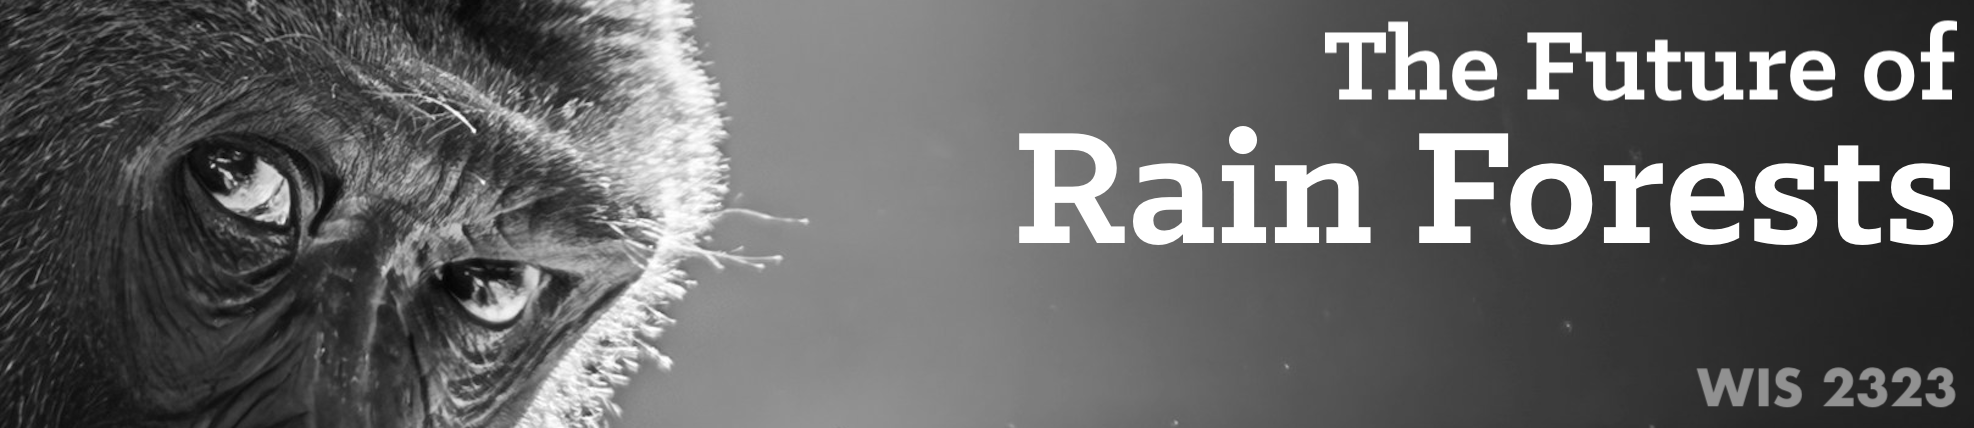
\includegraphics[keepaspectratio]{images/banner.png}}

This course investigates the fundamental issues addressed by scientists
studying tropical rain forests, including what gave rise to their
remarkable biodiversity, the drivers and consequences of deforestation,
why people are fascinated by rain forests, cultural and ecological
stereotypes about the tropics, and different approaches to forest
conservation and sustainability. \textbf{\emph{By the end of the course
students will be able to:}}

\begin{itemize}
\tightlist
\item
  Recognize and describe stereotypes about rain forests \& their
  residents
\item
  Analyze rain forest tropes in art, literature, \& popular culture
\item
  Discuss \& evaluate hypotheses for the origins and maintenance of
  tropical biodiversity
\item
  Explain \& compare the history and ecological influence of humans in
  rain forests
\item
  Review contemporary threats to rain forests
\item
  Analyze and visualize data on deforestation
\item
  Review and contrast strategies for rain forest conservation \&
  restoration
\item
  Identify rain forests in their daily lives \& set personal goals for
  advancing their conservation
\item
  Produce materials for communicating about tropical biology \&
  conservation to family and peers
\end{itemize}

\subsection*{When \& Where}\label{when-where}
\addcontentsline{toc}{subsection}{When \& Where}

\textbf{When:} Tuesdays 3:00-3:50 and Thursdays 3:00-4:55\\
\textbf{Where:} LIT 0231 (both days)

\subsection*{Instructor \& TA}\label{instructor-ta}
\addcontentsline{toc}{subsection}{Instructor \& TA}

\textbf{Instructor:} Dr.~Emilio M. Bruna {[}embruna@ufl.edu, (352)
846-0634{]}\\
\textbf{Teaching Assistant:} Priyanka Hari Haran {[}phariharan1@ufl.edu,
(352) 846-0527{]}

\subsection*{Credits \& Prerequisites}\label{credits-prerequisites}
\addcontentsline{toc}{subsection}{Credits \& Prerequisites}

\textbf{Credits:} 3\\
\textbf{Prerequisites:} None\\
\textbf{Quest Program:} Quest 2 \\
\textbf{GenEd Designation:} International

A minimum grade of C is required for Quest and General Education credit.
Courses intended to satisfy Quest and General Education requirements
cannot be taken S-U.

\subsection*{Minors \& Certificates}\label{minors-certificates}
\addcontentsline{toc}{subsection}{Minors \& Certificates}

This course counts towards:

\begin{itemize}
\tightlist
\item
  The Minor \& Certificate in Latin American Studies. See
  \url{https://www.latam.ufl.edu/academics/undergraduate-programs} for
  more information.
\end{itemize}

\bookmarksetup{startatroot}

\chapter{Required Materials}\label{required-materials}

\textbf{Materials and Supplies Fees}: None.

\textbf{Textbooks to purchase:} None.

\begin{itemize}
\item
  All materials, including readings and videos, will be made available
  on the course Canvas page. \bigskip
\item
  \emph{Students should sign up for free online access to the New York
  Times and Wall Street Journal by following the instructions at
  \href{https://businesslibrary.uflib.ufl.edu/c.php?g=943928&p=7708734}{this
  UF Libraries Website}} \footnote{Some of the assigned readings from
    these sources have dynamic multimedia data visualizations or video
    that can't be appreciated in the \texttt{.pdf} versions posted to
    canvas.}.
\end{itemize}

\begin{center}\rule{0.5\linewidth}{0.5pt}\end{center}

\bookmarksetup{startatroot}

\chapter{Office Hours}\label{office-hours}

\subsection*{When}\label{when}
\addcontentsline{toc}{subsection}{When}

\begin{itemize}
\item
  \textbf{Instructor:} Wednesday 1:30-3:30 (in-person and via Zoom, see
  below for details). You can drop by any time during the session, but
  if you want to guarantee a specific time slot you can do so by signing
  up here: \url{https://embruna.youcanbook.me/}. If you can't make it
  during the regularly scheduled office hours, you can send a message
  via Canvas to set up an appointment.
\item
  \textbf{Teaching Assistant:} Tuesday 4:00-5:30 pm (in-person \&
  online) or by appointment.
\end{itemize}

\subsection*{Where}\label{where}
\addcontentsline{toc}{subsection}{Where}

\begin{itemize}
\item
  \textbf{In-person:} The Tropical Ecology \& Conservation Lab. The lab
  is located at 711 Newell Drive next to Rawlings Hall (between the bus
  stop and the parking garage). For directions you can use this
  \href{https://maps.app.goo.gl/xo13vJmj8WXAivpZ9}{link to the lab on
  Google Maps}.
\item
  \textbf{Online:} To join Office Hours virtually use the Zoom
  Conferences link on the main menu of the course Canvas page. We are
  online the entire session.
\end{itemize}

\begin{tcolorbox}[enhanced jigsaw, bottomtitle=1mm, colback=white, colbacktitle=quarto-callout-tip-color!10!white, arc=.35mm, leftrule=.75mm, coltitle=black, colframe=quarto-callout-tip-color-frame, bottomrule=.15mm, breakable, toprule=.15mm, rightrule=.15mm, titlerule=0mm, title=\textcolor{quarto-callout-tip-color}{\faLightbulb}\hspace{0.5em}{Can you give me \textbf{one good reason} why I should go to Office
Hours?}, toptitle=1mm, left=2mm, opacitybacktitle=0.6, opacityback=0]

I can give you \textbf{ten}.

\begin{enumerate}
\def\labelenumi{\arabic{enumi}.}
\tightlist
\item
  To introduce yourself.
\item
  Get clarification on assignments.
\item
  Argue about a topic that came up in class.
\item
  Grab a (free) tea, coffee, or espresso in our lab kitchen.
\item
  Make sure you understood the key points from a class session.
\item
  Ask for feedback on ideas for course projects.
\item
  Get advice on successfully navigating academic life at UF.
\item
  Discuss how to gain experience for your post-graduation goals.
\item
  Request help arranging a study group.
\item
  You don't need a good reason\ldots just come on by.
\end{enumerate}

\end{tcolorbox}

\begin{center}\rule{0.5\linewidth}{0.5pt}\end{center}

\bookmarksetup{startatroot}

\chapter{Grades \& Attendance}\label{grades-attendance}

Learning in our class is achieved with an diverse array of methods
ranging from data analysis to essays to projects. In most class sessions
you will also be working with small groups of students to complete an
in-class assignment that reinforces the major themes of the day's topic.
In keeping with the philosophy of the Quest program, this course also
has \emph{Experiential Learning and Self-Reflection Components}.

\begin{tcolorbox}[enhanced jigsaw, bottomtitle=1mm, colback=white, colbacktitle=quarto-callout-tip-color!10!white, arc=.35mm, leftrule=.75mm, coltitle=black, colframe=quarto-callout-tip-color-frame, bottomrule=.15mm, breakable, toprule=.15mm, rightrule=.15mm, titlerule=0mm, title=\textcolor{quarto-callout-tip-color}{\faLightbulb}\hspace{0.5em}{Important note regarding class discussions \& group work.}, toptitle=1mm, left=2mm, opacitybacktitle=0.6, opacityback=0]

We will explore some challenging, important problems and increase our
understandings of different perspectives and approaches for addressing
them. These conversations may not always be easy; we sometimes will make
mistakes in both how we communicate our perspective and what we hear
other say. There may be times when we need patience, courage,
imagination, and of course mutual respect to engage our texts,
classmates, instructors, guests, and our own ideas and experiences.
\emph{Disrespectful or disruptive behavior will not be tolerated}. And
always remember that as scholars we rely on critical thinking, data,
prior scholarship, and expert opinion when interrogating assigned
readings and discussing course content with classmates and instructors.

\end{tcolorbox}

\subsection*{Assignments (1000 pts)}\label{assignments-1000-pts}
\addcontentsline{toc}{subsection}{Assignments (1000 pts)}

\begin{center}
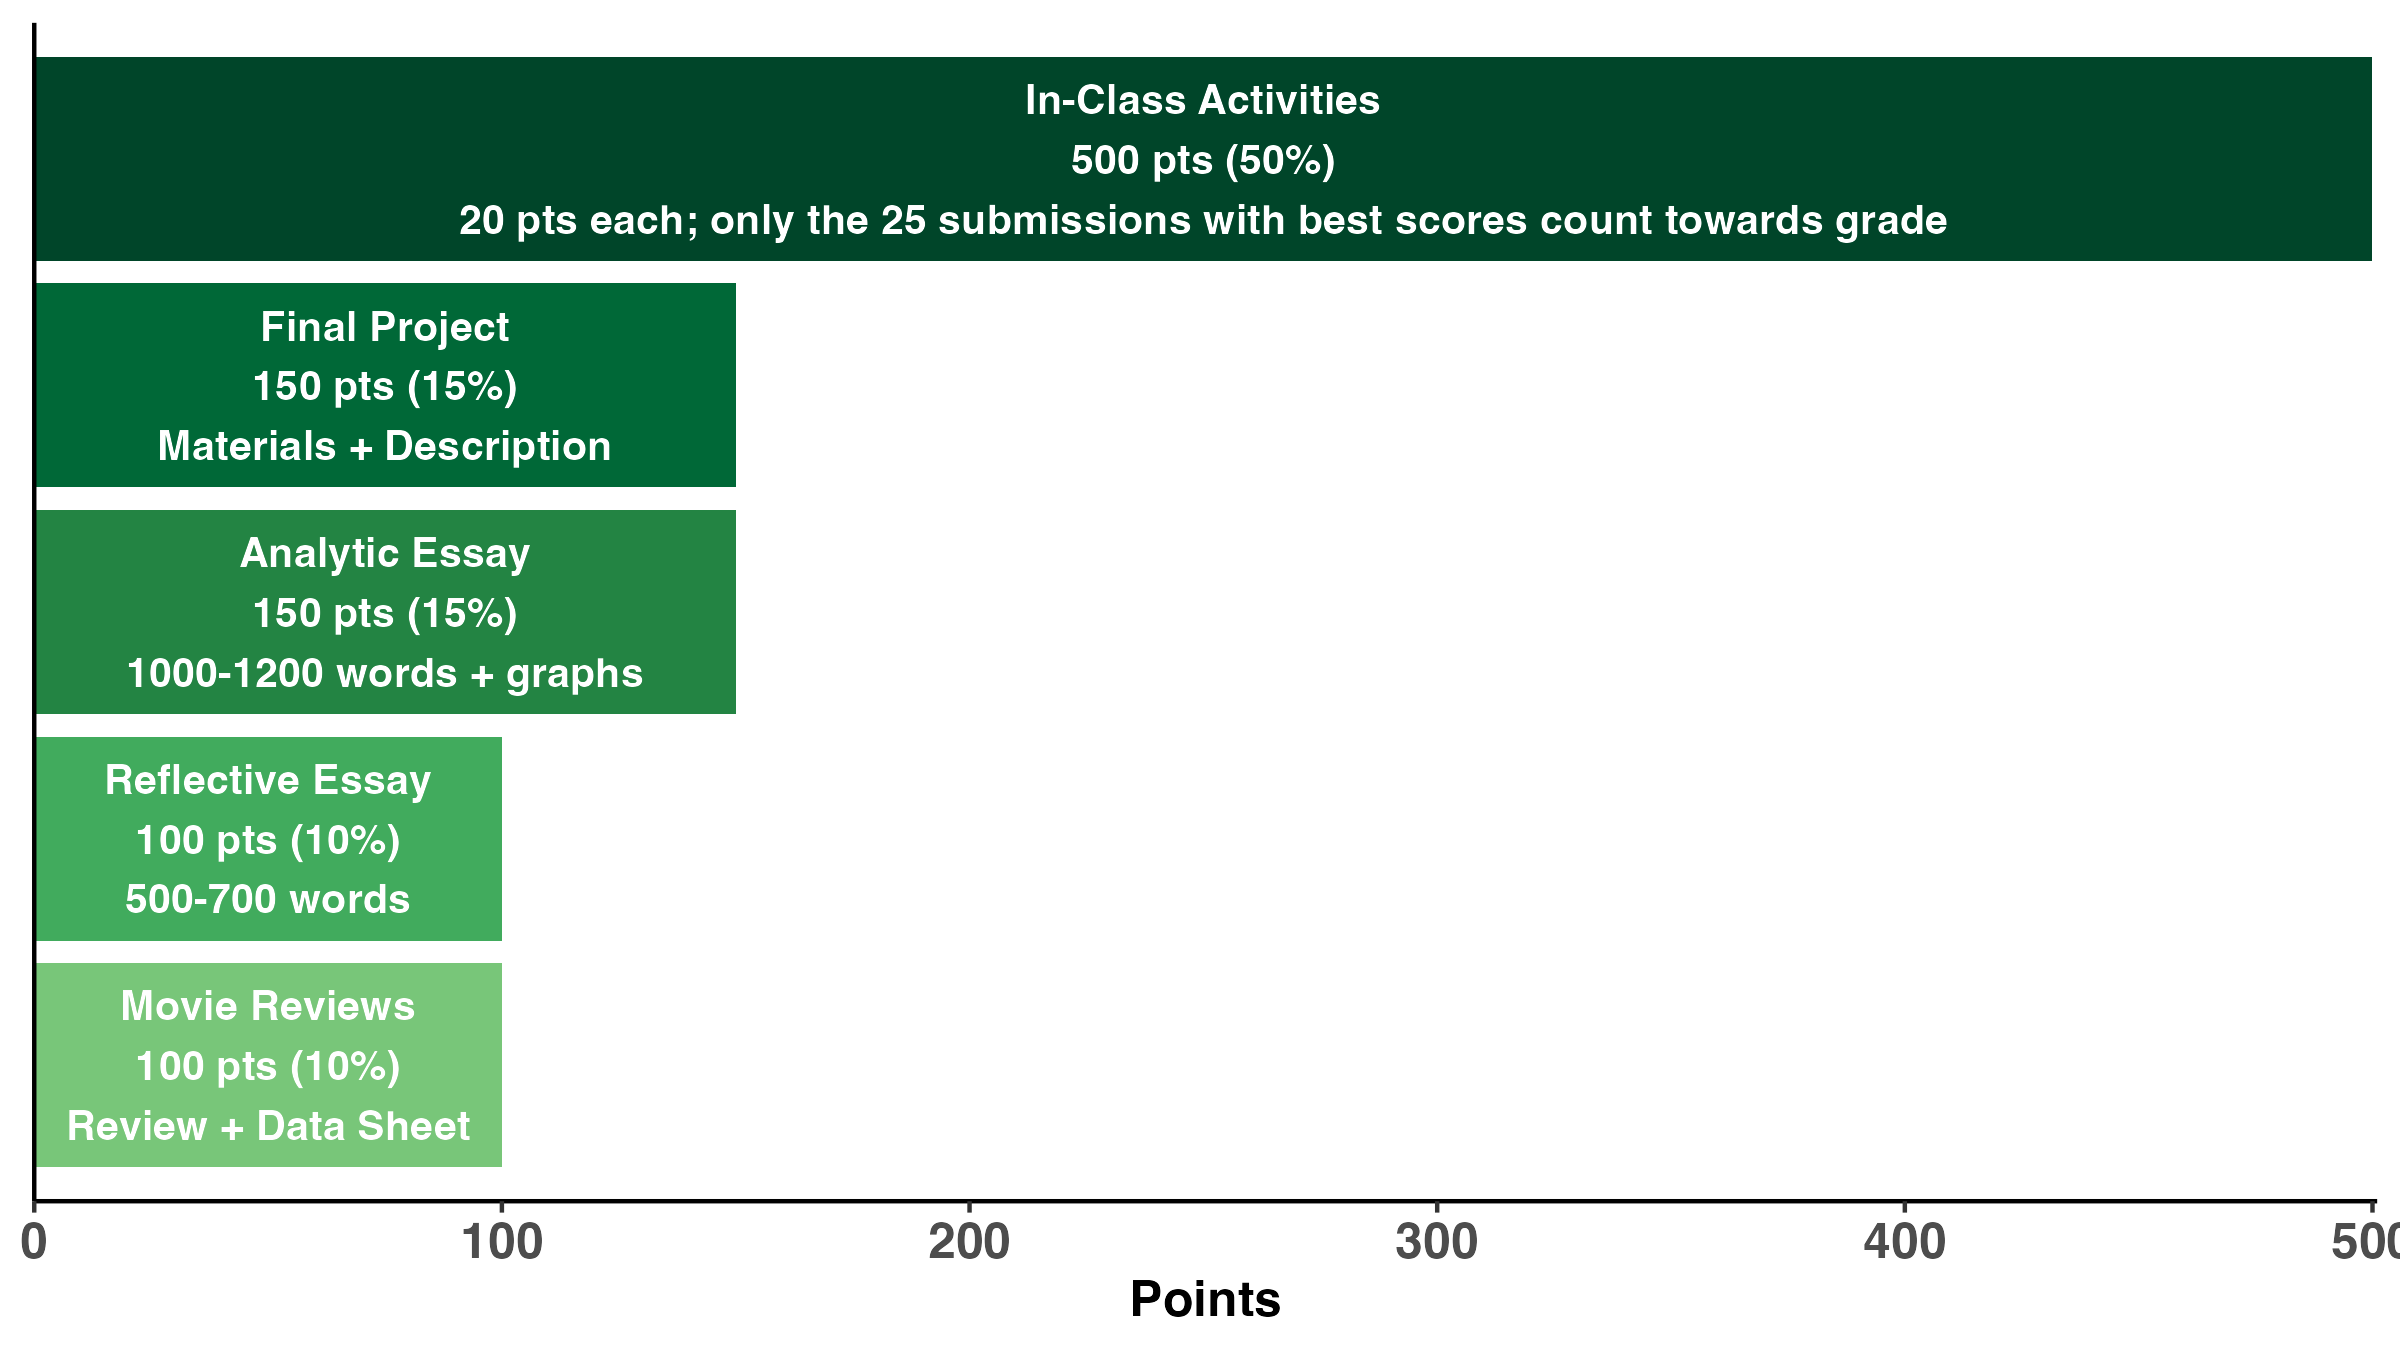
\includegraphics[width=1\linewidth,height=\textheight,keepaspectratio]{images/hw.png}
\end{center}

\subsection*{Grading}\label{grading}
\addcontentsline{toc}{subsection}{Grading}

\textbf{In-class Assignments are due by the following class session.}
Late assignments will lose 10 pts.

\textbf{\emph{Regrades:}} Requests for re-evaluation of assignments must
be accompanied by an explanation for why you think you deserve
additional credit and the number of additional points you think you
deserve. The deadline for submission is one week after the work was
returned.

\textbf{\emph{Grade Assignment}} (based on \% of total points earned): A
= 94--100\%, A- = 90--93\%, B+ = 87--89\%, B = 84--86\%, B- = 80--83\%,
C+ = 77--79\%, C = 74--76\%, C- = 70--73\%, D+ = 67--69\%, D = 64--66\%,
D- = 60--63\%, E\textless60

\textbf{\emph{Grade Points:}} For information on how UF assigns grade
points, visit:
\url{https://catalog.ufl.edu/UGRD/academic-regulations/grades-grading-policies/}

\subsection*{Attendance}\label{attendance}
\addcontentsline{toc}{subsection}{Attendance}

Though attendance is not required, many of the sessions we will be
completing activities in class that count towards your grade. Some these
can be completed independently, but by doing them in class you will
benefit from working collaboratively with the other students.
\textbf{Not all in-class activities can be completed independently.}
That is why only a subset of the in-class assignments count towards your
grade. We also offer some opportunities for extra credit.
\textbf{\emph{If you need to miss class for any reason, please let me
know as soon as possible}}. We will try to make arrangements for you to
complete any assignments and go over any material you will be missing.

\subsection*{Participation}\label{participation}
\addcontentsline{toc}{subsection}{Participation}

Consistent informed, thoughtful, and considerate class participation is
encouraged (and in some cases required). \emph{If you have personal
issues that prohibit you from joining freely in class discussion (e.g.,
shyness, language barriers, medical condition): no problem.} let us know
and we will discuss alternative modes of participation.

\begin{center}\rule{0.5\linewidth}{0.5pt}\end{center}

\bookmarksetup{startatroot}

\chapter{Calendar \& Key Dates}\label{calendar-key-dates}

\begingroup\fontsize{9}{11}\selectfont

\begin{longtable*}[l]{>{}c>{\centering\arraybackslash}p{7em}>{\raggedright\arraybackslash}p{25em}>{}r}
\toprule
\cellcolor[HTML]{1F691B}{\textcolor{white}{\textbf{WEEK}}} & \cellcolor[HTML]{1F691B}{\textcolor{white}{\textbf{DATE}}} & \cellcolor[HTML]{1F691B}{\textcolor{white}{\textbf{TOPIC}}} & \cellcolor[HTML]{1F691B}{\textcolor{white}{\textbf{ASSIGNMENT INFO}}}\\
\midrule
\addlinespace[0.3em]
\multicolumn{4}{l}{\textbf{WHY ARE WE FASCINATED BY TROPICAL RAIN FORESTS?}}\\
\textbf{\hspace{1em}Week 1} & 19-Aug & Class Starts Thursday! & \textbf{}\\
\textbf{\hspace{1em}} & 21-Aug & Course Welcome and Introduction & \textbf{}\\
\midrule\\
\textbf{\hspace{1em}Week 2} & 26-Aug & Historical Narratives & \textbf{}\\
\textbf{\hspace{1em}} & 28-Aug & Historical Narratives, cont. & \textbf{}\\
\midrule\\
\textbf{\hspace{1em}Week 3} & 2-Sep & Rain forests in Art \& Lit & \textbf{}\\
\textbf{\hspace{1em}} & 4-Sep & The Rain Forest in Pop Culture & \textbf{Movie Reviews Assigned}\\
\midrule\\
\addlinespace[0.3em]
\multicolumn{4}{l}{\textbf{THE ECOLOGY \& EVOLUTION OF TROPICAL RAIN FORESTS}}\\
\textbf{\hspace{1em}Week 4} & 9-Sep & What is a Rain Forest? & \textbf{}\\
\textbf{\hspace{1em}} & 11-Sep & What else is a Rain Forest? & \textbf{}\\
\midrule
\textbf{\hspace{1em}Week 5} & 16-Sep & Patterns of biodiversity 1 & \textbf{}\\
\textbf{\hspace{1em}} & 18-Sep & Patterns of biodiversity 2 & \textbf{}\\
\midrule\\
\textbf{\hspace{1em}Week 6} & 23-Sep & Origins of tropical biodiversity & \textbf{}\\
\textbf{\hspace{1em}} & 25-Sep & Maintenance of tropical biodiversity & \textbf{}\\
\midrule\\
\textbf{\hspace{1em}Week 7} & 30-Sep & Humans in rain forests 1 & \textbf{}\\
\textbf{\hspace{1em}} & 2-Oct & Humans in rain forests 2 & \textbf{Movie Reviews Due}\\
\midrule\\
\textbf{\hspace{1em}Week 8} & 7-Oct & Paradox of Luxuriance \& (Bio)Narratives Revisited & \textbf{}\\
\textbf{\hspace{1em}} & 9-Oct & JUNGLE FILM FEST (7 pm) & \textbf{}\\
\midrule
\addlinespace[0.3em]
\multicolumn{4}{l}{\textbf{THE DRIVERS AND IMPACTS OF DEFORESTATION}}\\
\textbf{\hspace{1em}Week 9} & 14-Oct & How much rain forest is there? & \textbf{Analytic Essay Assigned}\\
\textbf{\hspace{1em}} & 16-Oct & How much rain forest have we lost? & \textbf{}\\
\midrule
\textbf{\hspace{1em}Week 10} & 21-Oct & Drivers of deforestation 1 & \textbf{}\\
\textbf{\hspace{1em}} & 23-Oct & Drivers of deforestation 2 & \textbf{}\\
\midrule\\
\textbf{\hspace{1em}Week 11} & 28-Oct & Tropical forests and climate & \textbf{Analytic Essay Due}\\
\textbf{\hspace{1em}} & 30-Oct & Tropical forests and climate change & \textbf{Reflective Essay Assigned}\\
\midrule\\
\addlinespace[0.3em]
\multicolumn{4}{l}{\textbf{THE FUTURE OF TROPICAL RAIN FORESTS}}\\
\textbf{\hspace{1em}Week 12} & 4-Nov & Consumer choices & \textbf{}\\
\textbf{\hspace{1em}} & 6-Nov & Tropical Commodities \& DURIAN FEST & \textbf{}\\
\midrule
\textbf{\hspace{1em}Week 13} & 11-Nov & International conservation frameworks & \textbf{Reflective Essay Due}\\
\textbf{\hspace{1em}} & 13-Nov & Community-based Conservation & \textbf{Final Project Assigned}\\
\midrule\\
\textbf{\hspace{1em}Week 14} & 18-Nov & Tropical Rain Forests and Global Health & \textbf{}\\
\textbf{\hspace{1em}} & 20-Nov & Rain forest Headlines & \textbf{}\\
\midrule\\
\textbf{\hspace{1em}Week 15} & 25-Nov & No class - Thanksgiving & \textbf{}\\
\textbf{\hspace{1em}} & 27-Nov & No class - Thanksgiving & \textbf{}\\
\midrule\\
\textbf{\hspace{1em}Week 16} & 2-Dec & Protected Areas, Reforestation, Regeneration & \textbf{Final Project Due}\\
\textbf{} & 4-Dec & No Class - Reading Days & \textbf{}\\
\midrule\\
\textbf{Finals Week} & 9-Dec & No Final Exam & \textbf{}\\
\bottomrule
\end{longtable*}
\endgroup{}

\begin{center}\rule{0.5\linewidth}{0.5pt}\end{center}

\bookmarksetup{startatroot}

\chapter{FAQ}\label{faq}

\paragraph*{How do I contact the Instructor or
TA?}\label{how-do-i-contact-the-instructor-or-ta}
\addcontentsline{toc}{paragraph}{How do I contact the Instructor or TA?}

Send a message in CANVAS. That way both the TA and instructor will see
it and you will get a response more quickly (emails sent to us directly
tend to get buried under other messages).

\paragraph*{How will you send class
announcements?}\label{how-will-you-send-class-announcements}
\addcontentsline{toc}{paragraph}{How will you send class announcements?}

CANVAS. Check the course page for announcements and be sure you are
receiving Canvas emails and updates.

\paragraph*{What work should we complete BEFORE
class?}\label{what-work-should-we-complete-before-class}
\addcontentsline{toc}{paragraph}{What work should we complete BEFORE
class?}

Read, watch, listen to, or review all materials assigned for the
session. This material sets the stage for in-class activities.

\paragraph*{What will we do DURING
class?}\label{what-will-we-do-during-class}
\addcontentsline{toc}{paragraph}{What will we do DURING class?}

In-class exercises that reinforce key concepts, discussions of the
assigned readings, and let you practice skills in other assignments.
Some are completed individually, while others require working in groups
or pairs. Each activity will have instructions and a rubric; most are
designed to be finished in class.

\paragraph*{When is the ``in-class'' work
due?}\label{when-is-the-in-class-work-due}
\addcontentsline{toc}{paragraph}{When is the ``in-class'' work due?}

Deadlines are in Canvas, but typically the start of the next class
session.

\paragraph*{What if I miss class?}\label{what-if-i-miss-class}
\addcontentsline{toc}{paragraph}{What if I miss class?}

Attendance is not required, but in many of the sessions we will be
completing activities in class that count towards your grade. Some of
these can be completed independently, but by doing them in class you
will benefit from working collaboratively with the other students.
However, some of the in-class activities can not be completed on your
own. That's why only a subset of the in-class assignments count towards
your grade and we offer extra credit.

\paragraph*{I have to miss class on a certain date. What should I
do?}\label{i-have-to-miss-class-on-a-certain-date.-what-should-i-do}
\addcontentsline{toc}{paragraph}{I have to miss class on a certain date.
What should I do?}

Let us know as soon as possible so we can make arrangements for you to
review material you will miss and complete assignments.'')

\paragraph*{Class discussions are difficult for me. Will this affect my
grade?}\label{class-discussions-are-difficult-for-me.-will-this-affect-my-grade}
\addcontentsline{toc}{paragraph}{Class discussions are difficult for me.
Will this affect my grade?}

No! If there are issues that make engaging in discussions difficult
(e.g., shyness, language barriers, a medical condition), let us know and
we will find alternative modes of participation.

\paragraph*{I unexpectedly have no child care today\ldots what can I
do?}\label{i-unexpectedly-have-no-child-care-todaywhat-can-i-do}
\addcontentsline{toc}{paragraph}{I unexpectedly have no child care
today\ldots what can I do?}

UF does not have a policy on children in the classroom, so here is mine:
I never want students to feel they have to choose between their
responsibilities as parents and their education. Bringing your child to
class because of a gap in child care is totally fine (and that includes
babies). If you do so, please try and sit close to the exit so that you
can more easily step outside if you need to care for them and so other
students can continue learning.

\begin{center}\rule{0.5\linewidth}{0.5pt}\end{center}

\bookmarksetup{startatroot}

\chapter{UF Policies}\label{uf-policies}

\subsection*{Student Accomodations}\label{student-accomodations}
\addcontentsline{toc}{subsection}{Student Accomodations}

Students with disabilities or learning barriers that would like to
request academic accommodations should connect with the Disability
Resource Center by visiting
\url{https://disability.ufl.edu/students/get-started/}. Please share
your letter with me and discuss access needs as early as possible in the
semester so that I can do whatever is necessary to ensure your
participation and learning.

\subsection*{Course Evaluations}\label{course-evaluations}
\addcontentsline{toc}{subsection}{Course Evaluations}

Students are expected to provide professional and respectful feedback on
the quality of instruction in this course by completing course
evaluations. Guidance on how to provide constructive feedback is
available at \url{https://gatorevals.aa.ufl.edu/students/}. Students
will be notified when the evaluation period opens. Summaries of course
evaluation results are available to students at
\url{https://gatorevals.aa.ufl.edu/public-results/}. Students can
complete evaluations in three ways: (1) The email they receive from
GatorEvals, (2) Their Canvas course menu under GatorEvals, and (3) The
central portal at \url{https://my-ufl.bluera.com}.

\subsection*{University Honesty Policy}\label{university-honesty-policy}
\addcontentsline{toc}{subsection}{University Honesty Policy}

UF students are bound by The Honor Pledge which states, ``We, the
members of the University of Florida community, pledge to hold ourselves
and our peers to the highest standards of honor and integrity by abiding
by the Honor Code. On all work submitted for credit by students at the
University of Florida, the following pledge is either required or
implied: On my honor, I have neither given nor received unauthorized aid
in doing this assignment. The Honor Code
(\url{https://www.dso.ufl.edu/sccr/process/student-conduct-honor-code})
specifies a number of behaviors that are in violation of this code and
the possible sanctions. Furthermore, you are obligated to report any
condition that facilitates academic misconduct to appropriate personnel.
If you have questions or concerns, consult with the instructor or TAs.

\subsection*{Software Use}\label{software-use}
\addcontentsline{toc}{subsection}{Software Use}

All faculty, staff \& students are required \& expected to obey laws and
legal agreements governing software use. Failure to do so can lead to
monetary damages and/or criminal penalties for the individual violator.
Because such violations are also against UF policies \& rules,
disciplinary action will be taken as appropriate.

\subsection*{Attendance}\label{attendance-1}
\addcontentsline{toc}{subsection}{Attendance}

Requirements for class attendance \& make-up exams, assignments, and
other work are consistent with UF policies found at:
\url{https://catalog.ufl.edu/ugrad/current/regulations/info/attendance.aspx}.

\subsection*{In-Class Recording}\label{in-class-recording}
\addcontentsline{toc}{subsection}{In-Class Recording}

\textbf{Students are allowed to record video or audio of class lectures.
However, the purposes for which these recordings may be used are
strictly controlled.} The only allowable purposes are: \textbf{(1)} for
personal educational use, \textbf{(2)} in connection with a complaint to
the university, or \textbf{(3)} as evidence in, or in preparation for, a
criminal or civil proceeding. All other purposes are prohibited.
Specifically, students may not publish recorded lectures without the
written consent of the instructor. \textbf{\emph{A `class lecture' is:}}
an educational presentation intended to inform or teach enrolled
students about a particular subject, including any instructor-led
discussions that form part of the presentation, and delivered by any
instructor hired or appointed by the University, or by a guest
instructor, as part of a UF course. \textbf{\emph{A class lecture does
not include:}} lab sessions, student presentations, clinical
presentations such as patient history, academic exercises involving
solely student participation, assessments (quizzes, tests, exams), field
trips, private conversations between students in the class or between a
student and the faculty or lecturer during a class session.
\textbf{Publication without permission of the instructor is prohibited.
To `publish' means:} to share, transmit, circulate, distribute, or
provide access to a recording, regardless of format or medium, to
another person (or persons), including but not limited to another
student within the same class section. Additionally, a recording, or
transcript of a recording, is considered published if it is posted on or
uploaded to, in whole or in part, any media platform, including but not
limited to social media, book, magazine, newspaper, leaflet, or
third-party note/tutoring services. \textbf{\emph{A student who
publishes a recording without written consent may be subject to a civil
cause of action instituted by a person injured by the publication and/or
discipline under UF Regulation 4.040 Student Honor Code and Student
Conduct Code.}}

\begin{center}\rule{0.5\linewidth}{0.5pt}\end{center}

\bookmarksetup{startatroot}

\chapter{UF Student Resources}\label{uf-student-resources}

\subsection*{Health, Safety, \& Wellness}\label{health-safety-wellness}
\addcontentsline{toc}{subsection}{Health, Safety, \& Wellness}

\textbf{Wellness and Mental Health: }Students experiencing crises or
personal problems that interfere with their general well-being are
encouraged to utilize the university's counseling resources. The
Counseling \& Wellness Center provides confidential counseling services
at no cost for currently enrolled students. Resources are available on
campus for students having personal problems or lacking clear career or
academic goals, which interfere with their academic performance.
\emph{Visit \url{https://one.uf.edu/whole-gator/discover} for resources
that are designed to help you thrive physically, mentally, and
emotionally at UF.}

\begin{itemize}
\item
  \textbf{\emph{University Counseling \& Wellness Center:}} 3190 Radio
  Road, 352-392-1575. They can provide Counseling Services, Groups and
  Workshops, Outreach and Consultation, a Self-Help Library, and
  Wellness Coaching. \url{http://www.counseling.ufl.edu/}.
\item
  \textbf{\emph{U Matter, We Care:}} If you or someone you know is in
  distress, please contact
  \href{mailto:umatter@ufl.edu}{\nolinkurl{umatter@ufl.edu}},
  352-392-1575, or visit U Matter, We Care website
  (www.umatter.ufl.edu/) to refer or report a concern and a team member
  will reach out to the student in distress.
\end{itemize}

\textbf{Student Health Care Center:} Call 352-392-1161 for 24/7
information to help you find the care you need, or visit the Student
Health Care Center website.

\textbf{University Police Department:} Visit UF Police Department
website or call 352-392-1111 (or 9-1-1 for emergencies).

\textbf{UF Health Shands Emergency Room / Trauma Center:} For immediate
medical care call 352- 733-0111 or go to the emergency room at 1515 SW
Archer Road, Gainesville, FL 32608; Visit the UF Health Emergency Room
and Trauma Center website.

\textbf{Field and Fork Pantry:} The Hitchcock Pantry can provide food
and toiletries for students experi- encing food insecurity.
\url{https://pantry.fieldandfork.ufl.edu/}.

\subsection*{Academic Services}\label{academic-services}
\addcontentsline{toc}{subsection}{Academic Services}

\textbf{E-learning technical support: } Contact the UF Computing Help
Desk: (352) 392-4357 or
\href{mailto:helpdesk@ufl.edu}{\nolinkurl{helpdesk@ufl.edu}}.

\textbf{The Writing Studio} Help brainstorming, formatting, and writing
papers. Daytime (9:30am-3:30pm): 2215 Turlington Hall, 352-846-1138.
Evening (5:00pm-7:00pm): 1545 W University Avenue (Library West, Rm.
339).

\textbf{Career Connections Center} Reitz Union Ste 1300, (352) 392-1601.
Career assistance \& counseling services.

\textbf{Library Support} Various ways to receive assistance with respect
to using the libraries or finding resources. Call 866-281-6309 or email
\href{mailto:ask@ufl.libanswers.com}{\nolinkurl{ask@ufl.libanswers.com}}
for more information.

\textbf{Academic Resources} 1317 Turlington Hall, Call (352) 392-2010 or
to make a private appointment: 352- 392-6420. Email contact:
\href{mailto:teaching-center@ufl.edu}{\nolinkurl{teaching-center@ufl.edu}}.
General study skills and tutoring.

\textbf{Student Success Initiative} \url{http://studentsuccess.ufl.edu}.

\textbf{Student Complaints} Office of the Ombuds
\url{https://ombuds.ufl.edu/}; Visit the Complaint Portal webpage
\url{https://ombuds.ufl.edu/complaint-portal/} for more information.

\textbf{Enrollment Management Complaints (Registrar, Financial Aid,
Admissions)} View the Student Complaint Procedure webpage for more
information.

\textbf{UF Student Success Initiative} Visit
\url{https://studentsuccess.ufl.edu/} for resources that support your
success as a UF student.

\begin{center}\rule{0.5\linewidth}{0.5pt}\end{center}

\bookmarksetup{startatroot}

\chapter{Weekly Reading}\label{weekly-reading}

\begin{tcolorbox}[enhanced jigsaw, bottomtitle=1mm, colback=white, colbacktitle=quarto-callout-important-color!10!white, arc=.35mm, leftrule=.75mm, coltitle=black, colframe=quarto-callout-important-color-frame, bottomrule=.15mm, breakable, toprule=.15mm, rightrule=.15mm, titlerule=0mm, title=\textcolor{quarto-callout-important-color}{\faExclamation}\hspace{0.5em}{Important}, toptitle=1mm, left=2mm, opacitybacktitle=0.6, opacityback=0]

Please review the assigned material \textbf{\emph{before}} class.
\emph{Topics \& readings are subject to change based on current events;
changes will be announced via Canvas.}

\end{tcolorbox}

\section*{Week 1}\label{week-1}
\addcontentsline{toc}{section}{Week 1}

\markright{Week 1}

\paragraph*{1-2: Course Introduction}\label{course-introduction}
\addcontentsline{toc}{paragraph}{1-2: Course Introduction}

\begin{itemize}
\tightlist
\item
  None
\end{itemize}

\section*{Week 2}\label{week-2}
\addcontentsline{toc}{section}{Week 2}

\markright{Week 2}

\paragraph*{2-1: Historical Narratives}\label{historical-narratives}
\addcontentsline{toc}{paragraph}{2-1: Historical Narratives}

\begin{quote}
\emph{Goal: To introduce and discuss how historical narratives by the
first Europeans to visit the tropics have shaped contemporary
perceptions of tropical rain forests and the colonial roots of tropical
biology}
\end{quote}

\begin{itemize}
\tightlist
\item
  Excerpts from Historical Narratives {[}6 pages:
  \href{https://brunalab.github.io/wis2323_syllabus/readings/historical_narratives.pdf}{link}{]}
\end{itemize}

\paragraph*{2-2 Historical Narratives
(cont.);}\label{historical-narratives-cont.}
\addcontentsline{toc}{paragraph}{2-2 Historical Narratives (cont.);}

\begin{itemize}
\tightlist
\item
  none
\end{itemize}

\section*{Week 3}\label{week-3}
\addcontentsline{toc}{section}{Week 3}

\markright{Week 3}

\paragraph*{3-1 Rain Forest Imagery in Art \&
Literature}\label{rain-forest-imagery-in-art-literature}
\addcontentsline{toc}{paragraph}{3-1 Rain Forest Imagery in Art \&
Literature}

\begin{quote}
\emph{Goal: To see how the different depictions of the tropics and
tropical biodiversity from early European explorers are reflected in art
and literature.} readings/trf\_in\_lit\_and\_poetry.pdf
\end{quote}

\begin{itemize}
\item
  Excerpts from Literature/Poetry
  \href{https://brunalab.github.io/wis2323_syllabus/readings/trf_in_lit_and_poetry.pdf}{link}
  (5 pages)
\item
  Images of artwork {[}link{]} (4 pages)
\end{itemize}

\paragraph*{3-2 The Rain Forest in Pop
Culture}\label{the-rain-forest-in-pop-culture}
\addcontentsline{toc}{paragraph}{3-2 The Rain Forest in Pop Culture}

\begin{quote}
\emph{Goal: To compare the use and presentation of rain forest images by
the private sector and in different forms of popular culture, including
the film and music industries, and to evaluate how these depictions
influence perceptions of tropical countries \& people.}
\end{quote}

\begin{itemize}
\item
  Jolly, Priscilla. 2021. `Godzilla vs.~Kong': Monster movies evoke
  adventure but also `dangers' of tropics. \emph{The Conversation}.
  {[}\href{https://theconversation.com/godzilla-vs-kong-monster-movies-evoke-adventure-but-also-dangers-of-tropics-158105}{link
  to read online}{]} (4 pages)
\item
  Rose, Steve. 2016. ``From Tarzan to Avatar: the problem with `the
  white man in the jungle'\,''. The Guardian
  {[}\href{https://www.theguardian.com/film/2016/jul/06/why-the-white-man-in-the-jungle-film-wont-die}{link
  to read online}{]} (newspaper story, 5-10 min. read)
\end{itemize}

\section*{Week 4}\label{week-4}
\addcontentsline{toc}{section}{Week 4}

\markright{Week 4}

\paragraph*{4-1 What is a rain forest}\label{what-is-a-rain-forest}
\addcontentsline{toc}{paragraph}{4-1 What is a rain forest}

\begin{quote}
\emph{Goal: To learn the different ways biologists define the
``tropics'' and how the structure and dynamics of tropical rain forests
differ from those of forests in other parts of the world.}
\end{quote}

\begin{itemize}
\item
  Why Does Earth Have Deserts?
  {[}\href{https://www.youtube.com/watch?v=T6Us1sPXBfA}{link to
  video}{]}; 2 min long{]}
\item
  Emma Napper, British Broadcasting Corporation, ZDF, T., Tencent, \&
  France Télévisions (Producers), \& Napper, E. (Director). (2016).
  Jungles. {[}Video/DVD{]} BBC Worldwide. Retrieved from
  \url{https://video.alexanderstreet.com/watch/Jungles-2}
\end{itemize}

\paragraph*{4-2 What else is a Rain
Forest?}\label{what-else-is-a-rain-forest}
\addcontentsline{toc}{paragraph}{4-2 What else is a Rain Forest?}

\begin{quote}
\emph{Goal: To understand the geological history of tropical rain
forests, how climate, fire, and geological history drive the tipping
point between forests and savannas, and how this biogeographic,
geological, and climatic history shaped the evolution of tropical plants
and animals}
\end{quote}

\begin{itemize}
\tightlist
\item
  ``Ch. 4: Finding animals in the rainforest'' from Kricher, J.C.
  (2017). The new neotropical companion. In The New Neotropical
  Companion. Princeton Univ. Press (13 pp)
\end{itemize}

\section*{Week 5}\label{week-5}
\addcontentsline{toc}{section}{Week 5}

\markright{Week 5}

\paragraph*{5-1 Patterns of Biodiversity
1}\label{patterns-of-biodiversity-1}
\addcontentsline{toc}{paragraph}{5-1 Patterns of Biodiversity 1}

\begin{quote}
\emph{Goal: To observe and catalog the diversity of plant and animal
life forms that can be found in rain forests, to quantify the local
patterns of species richness and abundance in a tropical forest, and
compare these patterns with those in the temperate zone}
\end{quote}

\begin{itemize}
\tightlist
\item
  Ingrid Kvale, \& British Broadcasting Corporation (Producers), \&
  Kvale, I. (Director). (2021). Borneo: Sacred Forest. {[}Video/DVD{]}
  BBC Worldwide. Retrieved from
  \url{https://video.alexanderstreet.com/watch/borneo-sacred-forest}
\end{itemize}

\paragraph{5-2:}\label{section}

\begin{quote}
\emph{Goal: To understand global patterns of species richness and how
these vary from the tropics to the temperate zone}
\end{quote}

\begin{itemize}
\item
  We will be using iNaturalist in class. Read this: Matthew Earl Boone
  and Mathieu Basille. Using iNaturalist to contribute your nature
  observations to science. UF EDIS Document WEC413)
  \url{https://journals.flvc.org/edis/article/view/107698/110114}\ldots{}
\item
  \ldots and then familiarize yourself in advance by reviewing the
  iNaturalist website \url{https://www.inaturalist.org/}
\end{itemize}

\section*{Week 6}\label{week-6}
\addcontentsline{toc}{section}{Week 6}

\markright{Week 6}

\paragraph*{6-1: The Origins of Tropical
Biodiversity,}\label{the-origins-of-tropical-biodiversity}
\addcontentsline{toc}{paragraph}{6-1: The Origins of Tropical
Biodiversity,}

\begin{quote}
\emph{Goal: To review hypothesized mechanisms for the origins of
tropical diversity and the role of interspecific interactions in the
(co)evolution and diversification of tropical biodiversity}
\end{quote}

\begin{itemize}
\item
  ``Ch. 3: The Realm of Plants'' from Kricher, J. C. (2017). The new
  neotropical companion. In The New Neotropical Companion. Princeton
  University Press. (18 pp).
\item
  Is this the biggest flower in the world? ``BBC Earth: Corpse Flower
  Stinks of Death''
  {[}\href{https://www.youtube.com/watch?v=YxIpl38rsMo}{link to video},
  4 min long{]}.
\item
  A slightly less dramatic video in which you can get a better idea of
  the flower's size:
  {[}\href{https://www.youtube.com/watch?v=0cGRujABwuQ}{here}, 3 min
  long{]}
\item
  Maybe this is the biggest flower: The Titan arum
  {[}\href{https://www.youtube.com/watch?v=5Jg-GlCXpEI}{link to video},
  2 min long{]}
\end{itemize}

\paragraph*{6-2: The maintencnace of tropical
biodiversity}\label{the-maintencnace-of-tropical-biodiversity}
\addcontentsline{toc}{paragraph}{6-2: The maintencnace of tropical
biodiversity}

\begin{quote}
\emph{Goal: To review the biotic and abiotic mechanisms in tropical rain
forests that permit the coexistence of so many species.}
\end{quote}

\begin{itemize}
\item
  An introduction to Army Ants:
  {[}\href{https://www.youtube.com/watch?v=p16g5IVCdeE}{link to video},
  9 min long{]}.
\item
  See also this Army Ant Video by the BBC:
  {[}\href{https://www.youtube.com/watch?v=JsfiUR0ZzLw}{link to video},
  3 min long{]}.
\item
  A closer look at the Army Ant Birds:
  {[}\href{https://www.youtube.com/watch?v=SQPcIYV_vKM}{link to video},
  14 min long{]}.
\end{itemize}

\section*{Week 7}\label{week-7}
\addcontentsline{toc}{section}{Week 7}

\markright{Week 7}

\paragraph*{7-1 Humans are Part of Rain
Forests}\label{humans-are-part-of-rain-forests}
\addcontentsline{toc}{paragraph}{7-1 Humans are Part of Rain Forests}

\begin{quote}
\emph{Goal: To understand the history of human occupation of rain
forests including the contemporary demographic transition from rural to
urban occupation; to review the different ways in which humans have
historically modified rain forests and how this has shaped current rain
forest biodiversity.}
\end{quote}

\begin{itemize}
\tightlist
\item
  Kristine Allington, Michael Amundson, Linithd Aparicio, \& Caitlin
  Saks (Producers), \& Townsley, G. (Director). (2023). Ancient Builders
  of the Amazon. {[}Video/DVD{]} Public Broadcasting Service. Retrieved
  from
  \url{https://video.alexanderstreet.com/watch/ancient-builders-of-the-amazon}
\end{itemize}

\paragraph*{7-2 Humans are Part of Rain Forests
(Continued)}\label{humans-are-part-of-rain-forests-continued}
\addcontentsline{toc}{paragraph}{7-2 Humans are Part of Rain Forests
(Continued)}

\begin{quote}
\emph{Goal: To understand the history of human occupation of rain
forests including the contemporary demographic transition from rural to
urban occupation; to review the different ways in which humans have
historically modified rain forests and how this has shaped current rain
forest biodiversity.}
\end{quote}

\begin{itemize}
\tightlist
\item
  None
\end{itemize}

\section*{Week 8}\label{week-8}
\addcontentsline{toc}{section}{Week 8}

\markright{Week 8}

\paragraph*{8-1 Paradox of Luxuriance \& (Bio)Narratives
Revisited}\label{paradox-of-luxuriance-bionarratives-revisited}
\addcontentsline{toc}{paragraph}{8-1 Paradox of Luxuriance \&
(Bio)Narratives Revisited}

\begin{quote}
\emph{Goal: To understand how such a productive biome can be built on
such low-quality soils, and explore the implications of this ``Paradox
of Luxuriance''.}
\end{quote}

\begin{enumerate}
\def\labelenumi{\arabic{enumi}.}
\item
  \textbf{\emph{Watch:}} Anthony Bourdain's Parts Unknown: Congo (S1E8)
  {[}\href{https://www.youtube.com/watch?v=k59ToTXOuuE}{link to video},
  50 min long{]}.
\item
  \textbf{\emph{Read:}} Bourdain's Field Notes: Congo
  {[}\href{https://explorepartsunknown.com/congo/bourdains-field-notes-congo/}{read
  online}, 5 min read{]}.
\end{enumerate}

\paragraph{8-2}\label{section-1}

\section*{Week 9}\label{week-9}
\addcontentsline{toc}{section}{Week 9}

\markright{Week 9}

\paragraph*{9-1 How much tropical rain forest is
there?}\label{how-much-tropical-rain-forest-is-there}
\addcontentsline{toc}{paragraph}{9-1 How much tropical rain forest is
there?}

\begin{quote}
*Goal: To learn how forest cover is defined and estimated and how it
varies globally*
\end{quote}

\begin{itemize}
\item
  Louis Lucero II. New Interactive Tool Helps Track Earth's Forests
  {[}\href{https://www.nytimes.com/2013/11/15/science/earth/new-interactive-tool-helps-track-earths-forests.html}{NYTimes},
  10 min read{]}.
\item
  Nolen, Stephanie (Reporting) with Elkaim, Aaron Vincent (Photographs).
  2018. ``Inside the Amazon's Deforestation Crisis''. The Globe and
  Mail.
  {[}\href{https://www.theglobeandmail.com/news/world/amazon-rainforest-deforestation-crisis/article37722932/}{read
  online}, 20 min read{]}.
\end{itemize}

\paragraph*{9-2 How much tropical rain forest have we
lost?}\label{how-much-tropical-rain-forest-have-we-lost}
\addcontentsline{toc}{paragraph}{9-2 How much tropical rain forest have
we lost?}

\begin{quote}
\emph{Goal: To use forest cover data to estimate rates of tropical
forest loss over time}
\end{quote}

\begin{itemize}
\tightlist
\item
  Manuela Andreoni 2023 ``Despite Global Pledges, Tree Loss Is Up
  Sharply in Tropical Forests''
  {[}\href{https://www.nytimes.com/2023/06/27/climate/trees-tropical-forests-deforestation.html}{read
  online}, 10 min read{]}
\end{itemize}

\section*{Week 10}\label{week-10}
\addcontentsline{toc}{section}{Week 10}

\markright{Week 10}

\paragraph*{10-1 Drivers \& Consequences of Deforestation Part
1}\label{drivers-consequences-of-deforestation-part-1}
\addcontentsline{toc}{paragraph}{10-1 Drivers \& Consequences of
Deforestation Part 1}

\begin{quote}
\emph{Goal: Learn (a) how deforestation and other human activities alter
the structure \& functioning of rain forests, and (b) compare how these
drivers differ between the African, American, and Asian tropics.}
\end{quote}

\begin{itemize}
\item
  Serkez, Yaryna. 2020. Every Place Under Threat. \emph{NY Times}.
  {[}\href{https://www.nytimes.com/interactive/2020/10/02/opinion/amazon-under-threat.html}{read
  online}, 10 min read{]}.
\item
  Andreoni, Manuela, Blacki Migliozzi, Pablo Robles and Denise Lu.
  Photographs by Victor Moriyama. 2022. ``The Illegal Airstrips Bringing
  Toxic Mining to Brazil's Indigenous Land''. \emph{NY Times}.
  {[}\href{https://www.nytimes.com/interactive/2022/08/02/world/americas/brazil-airstrips-illegal-mining.html}{read
  online}, 15 min read{]}.
\item
  Searcey, Dionne (reporting) and Gilbertson, Ashley (photographs). 2022
  ``Raft by Raft, a Rainforest Loses Its Trees'' \emph{NY Times}.
  {[}\href{https://www.nytimes.com/interactive/2022/06/14/climate/congo-rainforest-logging.html}{read
  online}, 10 min read{]}.
\end{itemize}

\paragraph*{10-2 Drivers \& Consequences of Deforestation Part
II}\label{drivers-consequences-of-deforestation-part-ii}
\addcontentsline{toc}{paragraph}{10-2 Drivers \& Consequences of
Deforestation Part II}

\begin{quote}
\emph{Goal: Continue learning (a) how deforestation and other human
activities alter the structure \& functioning of rain forests, and (b)
compare how these drivers differ between the African, American, and
Asian tropics.}
\end{quote}

\begin{itemize}
\item
  Devouring the Rain Forest. Washington Post.
  {[}\href{https://www.washingtonpost.com/world/interactive/2022/amazon-beef-deforestation-brazil/}{read
  online}, 20 min read{]}.
\item
  Robles, Pablo, Anuradha Raghu, Adam Majendie and Jin Wu 2021. ``The
  World's Addiction to Palm Oil Is Only Getting Worse''. Bloomberg News.
  {[}\href{https://www.bloomberg.com/graphics/2021-palm-oil-deforestation-climate-change/}{read
  online}, 10 min read{]}.
\item
  Mason, Margie \& McDowell, Robin. 2020. ``Palm oil labor abuses linked
  to world's top brands, banks''. Associated Press.
  {[}\href{https://apnews.com/article/virus-outbreak-only-on-ap-indonesia-financial-markets-malaysia-7b634596270cc6aa7578a062a30423bb}{read
  online}, 10 min read{]}.
\end{itemize}

\section*{Week 11}\label{week-11}
\addcontentsline{toc}{section}{Week 11}

\markright{Week 11}

\paragraph*{11-1 Tropical Forests \& Global
Climate}\label{tropical-forests-global-climate}
\addcontentsline{toc}{paragraph}{11-1 Tropical Forests \& Global
Climate}

\begin{quote}
\emph{Goal: Climate change and Tropical Forests To understand the
relationship between tropical forests, deforestation, and the global
climate cycle.}
\end{quote}

\begin{itemize}
\item
  BBC News: Amazon rainforest: `Once it's gone, it's gone forever'
  (interview with Erika Berenguer).
  {[}\href{https://www.youtube.com/watch?v=TigV80hwebg}{link to video},
  3 min long{]}.
\item
  Pearce, Fred. 2018. ``Rivers in the Sky: How Deforestation Is
  Affecting Global Water Cycles.'' Yale360.
  {[}\href{https://e360.yale.edu/features/how-deforestation-affecting-global-water-cycles-climate-change}{read
  online}, 10 min read{]}.
\end{itemize}

\paragraph*{11-2 Tropical Forests \& Climate
Change}\label{tropical-forests-climate-change}
\addcontentsline{toc}{paragraph}{11-2 Tropical Forests \& Climate
Change}

Henry Knight Lozano (2023) California and Florida grew quickly on the
promise of perfect climates in the 1900s -- today, they lead the country
in climate change risks. \emph{The Conversation}.
\href{https://theconversation.com/california-and-florida-grew-quickly-on-the-promise-of-perfect-climates-in-the-1900s-today-they-lead-the-country-in-climate-change-risks-207470}{Link}

\begin{itemize}
\tightlist
\item
  learn about the EN-ROADS simulator we will be using in class at this
  {[}\href{https://www.climateinteractive.org/en-roads/}{link to
  website}, 15 min read{]}. You can even start experimenting with it
  here:
  {[}\href{https://en-roads.climateinteractive.org/scenario.html?v=22.8.0}{link
  to site}{]}.
\end{itemize}

\section*{Week 12}\label{week-12}
\addcontentsline{toc}{section}{Week 12}

\markright{Week 12}

\paragraph*{12-1 Consumer Choices}\label{consumer-choices}
\addcontentsline{toc}{paragraph}{12-1 Consumer Choices}

\begin{quote}
\emph{Goal: To understand how global production and chains and consumer
demand in Europe and North America influence patterns of deforestation
in tropical countries.}
\end{quote}

\begin{itemize}
\item
  Carodenuto, Sophia. 2021. ``Chocolate fix: How the cocoa industry
  could end deforestation in West Africa''. \emph{The Conversation}.
  {[}\href{https://theconversation.com/chocolate-fix-how-the-cocoa-industry-could-end-deforestation-in-west-africa-161953}{read
  online}, 10 min read{]}.
\item
  Lawal,Shola. 2020. ``Our Endless Appetite For Chocolate Has Bitter
  Environmental Consequences'' Huffington Post.
  {[}\href{https://tinyurl.com/y6curgmn}{read online}, 10 min read{]}.
\item
  Williams, Wyatt. 2021. ``How Your Cup of Coffee Is Clearing the
  Jungle''. \emph{NY Times}.
  {[}\href{https://www.nytimes.com/2021/08/11/magazine/indonesia-rainforest-coffee.html}{read
  online}{]} Longer, but really gripping and the article includes a link
  to an audio version if you prefer to listen to it.
\item
  \textbf{\emph{Optional:}} Mufson, Steven and Georges, Salwan. 2019.
  ``The trouble with chocolate'' Washington Post
  {[}\href{https://www.washingtonpost.com/graphics/2019/national/climate-environment/mars-chocolate-deforestation-climate-change-west-africa/}{read
  online} to see the amazing maps, pictures, and data visualizations.
\end{itemize}

\paragraph*{12-2 Tropical Commodities \& DURIAN
FEST}\label{tropical-commodities-durian-fest}
\addcontentsline{toc}{paragraph}{12-2 Tropical Commodities \& DURIAN
FEST}

\begin{quote}
\emph{Goal: To learn about the global market in tropical fruit crops and
the economic impact of tropical fruit production in Florida.}
\end{quote}

\begin{itemize}
\item
  Weintraub, Karen. 2019. ``They're Smelly and Spiky, and They Need Bats
  to Pollinate Them''. \emph{NY Times}.
  {[}\href{https://www.nytimes.com/2019/12/04/science/bats-durians-indonesia.html}{read
  online}, 5 min read{]}.
\item
  Wharton, Rachel. 2020. How the Tip of Florida Became a Tropical-Fruit
  Paradise. Atlas Obscura.
  {[}\href{https://www.atlasobscura.com/articles/tropical-fruit-farms-in-united-states}{read
  online}, 5 min read{]}.
\end{itemize}

\begin{itemize}
\item
  Hunt, Chris and Premathilake, Rathnasiri. 2018. ``Prehistoric people
  started to spread domesticated bananas across the world 6,000 years
  ago.'' \emph{The Conversation}.
  {[}\href{https://theconversation.com/prehistoric-people-started-to-spread-domesticated-bananas-across-the-world-6-000-years-ago-99547}{read
  online}, 5 min{]}.
\item
  \textbf{\emph{Listen:}} NPR's Throughline Podcast: ``There Will Be
  Bananas''
  {[}\href{https://www.npr.org/2020/01/07/794302086/there-will-be-bananas}{listen
  online}, 56 min{]}.
\end{itemize}

\section*{Week 13}\label{week-13}
\addcontentsline{toc}{section}{Week 13}

\markright{Week 13}

\paragraph*{13-1 International Conservation
Frameworks}\label{international-conservation-frameworks}
\addcontentsline{toc}{paragraph}{13-1 International Conservation
Frameworks}

\begin{quote}
\emph{Goal: To learn about the major local, national, and multi-national
approaches to reducing deforestation by comparing their efficacy and
socioeconomic impacts. REDD and Payment for Ecosystem Services.}
\end{quote}

\begin{itemize}
\tightlist
\item
  UN-REDD Programme: An introduction to REDD+
  \href{https://www.un-redd.org/sites/default/files/2021-10/1.\%20Introduction\%20to\%20REDD\%2B_Tim\%20Christophersen.pdf}{link}.
\end{itemize}

\begin{quote}
Note: this is a slide deck designed to introduce the REDD+ framework to
a general audience. The content is exceptional, but don't just read the
material -- think about how it is being presented (graphics, etc.) and
if it effectively communicates their message. I've asked you do this not
just to prepare for today's lesson, but because it will be useful for
your Final Project (TL;dr\ldots the presentation is awful: busy slides,
too much text, overly complicated graphics\ldots we'll talk about how it
could be improved).
\end{quote}

\begin{itemize}
\tightlist
\item
  Ruth Maclean (reporting, writing), Caleb Kabanda (reporting), and
  Nanna Heitmann (photography). 2022. ``What do the protectors of
  Congo's peatlands get in return?'' \emph{NY Times}.
  {[}\href{https://www.nytimes.com/interactive/2022/02/21/headway/peatlands-congo-climate-change.html}{read
  online}, 10 min read{]}.
\end{itemize}

\paragraph*{13-2 Community based
conservation}\label{community-based-conservation}
\addcontentsline{toc}{paragraph}{13-2 Community based conservation}

\begin{quote}
\emph{Goal: To learn about how local communities are engaged in rain
forest conservation and sustainable development efforts in the tropics
and beyond.}
\end{quote}

\begin{itemize}
\tightlist
\item
  Kimbrough, L. 2021. ``How settlers, scientists, and a women-led
  industry saved Brazil's rarest primate''. Mongabay.com
  {[}\href{https://news.mongabay.com/2021/05/how-settlers-scientists-and-a-women-led-industry-saved-brazils-rarest-primate/}{read
  online}, 10 min read{]}.
\end{itemize}

Katrina Kosec et al.~(2025) Forest loss in Malawi: how having women at
the table affected debates and decisions about solutions. \emph{The
Conversation}. {[}{[}read online{]}
(https://theconversation.com/forest-loss-in-malawi-how-having-women-at-the-table-affected-debates-and-decisions-about-solutions-research-259699),
10 min read{]}.

\begin{itemize}
\item
  Don't underestimate what one person can do on their own: ``BBC World
  Service: The man who grew his own rainforest''
  {[}\href{https://www.youtube.com/watch?v=AngaeIf78AQ}{link to video},
  5 min long{]} (keep an eye out for the Euglossine bees we learned
  about earlier in the semester\ldots you can see them collecting
  scented oil from flowers at 2:04).
\item
  \textbf{Come prepared to make some money:} we're looking into the
  economic benefits of setting aside land (or not) for conservation. To
  prepare, review this document over before class:
  {[}\href{https://www.tandfonline.com/doi/full/10.1080/00220485.2016.1146098}{link},
  10-15 min read{]}.
\end{itemize}

\section*{Week 14}\label{week-14}
\addcontentsline{toc}{section}{Week 14}

\markright{Week 14}

\paragraph*{14-1 Tropical rain forests \& Global
Health}\label{tropical-rain-forests-global-health}
\addcontentsline{toc}{paragraph}{14-1 Tropical rain forests \& Global
Health}

\begin{quote}
\emph{Goal: To learn about the relationship between deforestation and
the emergence and spread of tropical diseases like Zika and Malaria from
the tropics to other regions of the globe}.
\end{quote}

\begin{itemize}
\tightlist
\item
  Vittor, Amy, Gabriel Zorello Laporta, and Maria Anice Mureb Sallum.
  2020. How deforestation helps deadly viruses jump from animals to
  humans. \emph{The Conversation}.
  {[}\href{https://theconversation.com/how-deforestation-helps-deadly-viruses-jump-from-animals-to-humans-139645}{read
  online}, 15 min read{]}.
\end{itemize}

UF EPI. (2024) Florida's mosquitoes can make you sick: Here's how to
protect yourself.
\href{https://epi.ufl.edu/2024/05/01/floridas-mosquitoes-can-make-you-sick-heres-how-to-protect-yourself/}{link}

\begin{itemize}
\item
  Kuchipudi, Suresh V. 2020. Why so many epidemics originate in Asia and
  Africa -- and why we can expect more. \emph{The Conversation}.
  {[}\href{https://theconversation.com/why-so-many-epidemics-originate-in-asia-and-africa-and-why-we-can-expect-more-131657}{read
  online}, 10 min{]}.
\item
  Lavinas Picq, Manuela 2020. ``Spreading Faith, and Disease''. \emph{NY
  Times}.
  {[}\href{https://www.nytimes.com/2020/10/02/opinion/amazon-missionaries-tribes-disease.html}{read
  online}, 15 min read{]}.
\end{itemize}

\paragraph*{14-2 Rain Forest Headlines}\label{rain-forest-headlines}
\addcontentsline{toc}{paragraph}{14-2 Rain Forest Headlines}

\begin{quote}
\emph{Goal: To learn how journalists based in different countries or
different global audiences chose and cover stories about rain forests
and deal with the risks of covering this beat}.
\end{quote}

\begin{itemize}
\tightlist
\item
  Nicas, Jack (reporting) and Moriyama,Victor (Photos, Video). 2022.
  Inside the Amazon Journey That Left a Journalist and an Activist Dead.
  \emph{NY Times}.
  {[}\href{https://www.nytimes.com/interactive/2022/07/11/world/americas/amazon-murder-dom-phillips-bruno-pereira.html?smid=tw-nytimes&smtyp=cur}{read
  online}, 15 min read{]}
\end{itemize}

\section*{Week 15}\label{week-15}
\addcontentsline{toc}{section}{Week 15}

\markright{Week 15}

\begin{itemize}
\tightlist
\item
  No Class - Thanksgiving Holiday
\end{itemize}

\section*{Week 16}\label{week-16}
\addcontentsline{toc}{section}{Week 16}

\markright{Week 16}

\paragraph*{16-1 Forest Restoration \&
Regeneration}\label{forest-restoration-regeneration}
\addcontentsline{toc}{paragraph}{16-1 Forest Restoration \&
Regeneration}

\begin{quote}
\emph{Goal 1: To learn the difference between passive regeneration and
active restoration and assess evidence for whether they can be used to
reverse the effects of deforestation}
\end{quote}

\begin{quote}
\emph{Goal 2: To learn about different global categories of protected
areas, the importance of protected areas in the tropics for conserving
forest, and how the threats to protected areas vary regionally and
globally.}
\end{quote}

\begin{itemize}
\tightlist
\item
  Dasgupta, Shreya (with research by Annika Schlemm \& Zuzana
  Burivalova). 2017. ``Do protected areas work in the tropics?''
  Mongabay.com.
  {[}\href{https://news.mongabay.com/2017/12/do-protected-areas-work-in-the-tropics/}{read
  online}, 25 min read{]}.
\end{itemize}

Matti Barthel et al.~(2025) DRC's plan for the world's largest tropical
forest reserve would be good for the planet: can it succeed? \emph{The
Conversation}. {[}{[}read online{]}
(https://theconversation.com/drcs-plan-for-the-worlds-largest-tropical-forest-reserve-would-be-good-for-the-planet-can-it-succeed-254394),
10 min read{]}.

\begin{itemize}
\tightlist
\item
  Medici, Patricia. 2015 TED Fellows Talk. ``The coolest animal you know
  nothing about\ldots and how we can save it''.
  {[}\href{https://www.ted.com/talks/patricia_medici_the_coolest_animal_you_know_nothing_about_and_how_we_can_save_it\#t-694653}{link
  to video}, 11:20 min long{]}.
\end{itemize}

\begin{itemize}
\tightlist
\item
  Jennifer Weeks. Ending Amazon deforestation: 4 essential reads about
  the future of the world's largest rainforest. \emph{The Conversation}
  \href{https://theconversation.com/ending-amazon-deforestation-4-essential-reads-about-the-future-of-the-worlds-largest-rainforest-194800}{link}
  (4 pages)
\end{itemize}

\newpage

\bookmarksetup{startatroot}

\chapter{Student Learning Objectives}\label{student-learning-objectives}

B = Biological Sciences, Q2 = Quest 2

\begin{tabular}[t]{>{\raggedright\arraybackslash}p{25em}>{\raggedright\arraybackslash}p{25em}l}
\toprule
\cellcolor[HTML]{1F691B}{\textcolor{white}{\textbf{CONTENT}}} & \cellcolor[HTML]{1F691B}{\textcolor{white}{\textbf{CONNECTION}}} & \cellcolor[HTML]{1F691B}{\textcolor{white}{\textbf{}}}\\
\em{\textbf{Students demonstrate competence in the terminology, concepts, theories, and methodologies used within the discipline(s)}} & \em{\textbf{\cellcolor{white}{\textcolor{black}{Students connect course content with meaningful critical reflection on their intellectual, personal, and professional development at UF and beyond.}}}} & \em{\textbf{}}\\
(1) Describe the evolutionary and ecological factors underlying the distribution of biodiversity in tropical rain forests. Assessments: In-class activities, Final Project. (B). 

(2)  Distinguish (a) the different ways humans use and alter rain forests, and (b) the social, economic, and biological consequences of these activities. Assessments: In-class activities, Reflective Essay, Final Project. (B, Q2)  

(3)  Explain how genetics, remote sensing, computational tools, and other scientific developments have advanced research on the ecology and evolution of rain forest biota. Assessments: In-class activities, Analytic Essay. (B). 

(4)  Examine the historical factors that have shaped cultural perceptions of rain forests. Assessments: In-class activities, Movie Reviews, Final project. (Q2).  

(5)  Analyze how narratives about rain forests are reflected in different types of contemporary cultural expression. Assessments: In-class activities, Movie Reviews, Final project. (Q2).  

(6)  Distinguish between the primary drivers of forest loss and how they vary geographically. Assessments: In-class activities, Analytic Essay. (B, Q2)  

(7)  Critique different proposed mechanisms for rain forest conservation. Assessments: In-class activities, Analytic Essay. (B, Q2) & (1) Examine the cultural, economic, and historical experiences of people in rain forest countries, how this compares with our preconceived notions of the same, and the consequences of this disparity for our scientific understanding of rain forests and their conservation. Assessments: In-class activities, Movie Reviews, Final Project  (Q2). 

(2) Assess the feedbacks between (a) the actions of individuals, governments, and the private sector, (b) global economic, social, and political conditions, and (c) the status rain forests and the global climate cycle. Assessments: In-class activities, Reflective Essay, Analytic Essay (Q2). 

(3) Appraise the ubiquity of tropical forest products in daily life, the role and impact of the global commodity chains that make this possible, and the consequences of consumer behavior for forest conservation and socioeconomic sustainability. Assessments: In-class activities, Final Project (Q2). 

(4) Analyze the local, regional, and global ecosystem services provided by tropical rain forests, how these vary geographically, and some of the cultural and ecological factors responsible for these differences. Assessments: In-class activities, Reflective Essay, Analytic Essay, Final Project (Q2). & \cellcolor{white}{\textcolor{black}{}}\\
\cellcolor[HTML]{1F691B}{\textcolor{white}{\textbf{COMMUNICATION}}} & \cellcolor[HTML]{1F691B}{\textcolor{white}{\textbf{CRITICAL THINKING}}} & \cellcolor[HTML]{1F691B}{\textcolor{white}{\textbf{}}}\\
\em{\textbf{Students communicate knowledge, ideas and reasoning clearly and effectively in written and oral forms appropriate to the discipline(s)}} & \em{\textbf{\cellcolor{white}{\textcolor{black}{Students carefully and logically analyze information from multiple perspectives and develop reasoned solutions to problems within the discipline(s).}}}} & \em{\textbf{}}\\
(1) Generate graphical analyses of quantitative data used to study rain forest biology and conservation (Q2, B). Assessments: In-class activities, Analytic Essay. 

(2) Compose summaries of  research on multidisciplinary questions relevant to tropical forest biology and conservation based on logical arguments (Q2, B). Assessments: In-class activities, Analytic Essay, Final Project. 

(3) Develop audience-specific content and materials with which to communicate an important issue related to tropical forest biology and conservation. Assessments: In-class activities,  Reflective Essay, Movie Reviews, Analytic Essay, Final Project (Q2). & (1) Test hypotheses regarding trends in deforestation and how forest regeneration varies geographically with quantitative data on forest cover and use news stories, primary literature, and other sources to propose mechanisms responsible for the patterns observed. Assessments: In-class activities, Analytic Essay  (B, Q2). 

(2) Analyze qualitative data on rural-urban migration and human demographic shifts in tropical countries and assess the potential implications of the results for conservation and broader societal issues. Assessments: In-class activities, Analytic Essay (B, Q2). 

(3) Explain the relationship between deforestation and the global climate cycle. Compare alternative policy pathways for reducing CO2 emissions using the En-ROADS global climate simulator. Assessments: In-class activities, Reflective Essay (B, Q2). & \cellcolor{white}{\textcolor{black}{}}\\
\bottomrule
\end{tabular}


\backmatter


\end{document}
